%************************************************
\chapter{Clustering and visualizing tissues from 3D single cell expression data}\label{ch:non_spatial_clustering_visualization} 
%************************************************
\section{Elements of clustering for biological tissues}
	\subsection{Motivations}
	Following the conclusions of the previous chapter \ref{ch:singlecell} in which was discussed the shift in the scale of study from the biological tissue to the single cell, and the main challenges to analyse and interpret such data, the first question that seems natural to answer is the following. Given single cell gene expression data only, is it possible to classify cells that are the most alike together in order to define the organization of complex biological tissues like the brain of \platyfull{}?\\
	
	This question fundamentally is a clustering or a classification problem. Indeed, small units need to be put in a determined number of classes or clusters because they are alike in one way or another. The question asked above actually contains several parts.\\
	
	 As anatomical and functional information about some tissues in the brain of \platy{} is already available (see chapter \ref{ch:background}), the obvious validation for any clustering/classification method developed is be to check that the single cell level information also leads to the definition of those known tissue. Once this has been validated, it seems important to determine whether the single cell expression data \emph{adds} to the known biology by redefining known tissues or find new ones. This already is a big challenge but the question can be pushed further. Indeed, as mentioned in chapter \ref{ch:background}, because gene expression is the key process in a cell's life, knowing what genes are specifically expressed in a novel or redefined tissue can help us understand what the function of this functional tissue is.

	\subsection{General considerations about clustering}
	I mentioned before that tools developed to answer those questions could be either be clustering or classification methods. In the field of machine learning, those two notions are fundamentally divergent. Indeed, when clustering describes a method that assigns points to an unknown number of sets, in an undirected way, classification takes advantage of an already known classification of points to classify, in a directed manner, new elements in a determined number of clusters.\\
	
	In my case, the number of tissues in the brain of \platy{} is unknown and there is no previous classification or a strong enough biological knowledge of each and every cell to opt for a directed classification. Therefore the methods presented hereafter will be clustering methods with respect to the machine learning definition of the word.\\
	
	As a general consideration about clustering, it is interesting to note that unless working on simple enough datasets, there is no perfect method, This is especially true when dealing with biological data, where the inner complexity and the noise level (see \ref{sec:quantitative_single_cell}} tend to be extremely high. \\
	
	To illustrate that notion, for the single cell expression data in \platy{}'s brain, the question of the finding the ``true" number of tissues is extremely complicated. Without any prior knowledge, the statistical methods to determine the number of clusters presented in this thesis will yield indications about what the optimal number ``tissues" is given the data, which does not necessarily means that this number is biologically true.\\
	
	For a complex dataset such as the brain of a complex organism, a crucial matter in the upstream and the downstream analysis is to be able to visualize the data. This is especially true when the considered tissue is in 3 3 dimensions. For example, an important part of the upstream analysis to clustering was to visualize the gene expression patterns in the brain to find the right binarization thresholds. In the downstream analysis, after developing a clustering method, seeing the resulting clusters and their localizations in the brain is crucial. Therefore, I decided to develop a tool for simple datasets 3D visualization taking advantage of the latest developments in browser based technologies.
	
	

\section{Visualizing clustering results in 3D with bioWeb3D}
	\subsection{Background}

Visualisation is a key challenge in the analysis of large biological datasets, especially when analysing organized structures with distinct sub-clusters \cite{Rubel10}. This is particularly important when analysing 3-Dimensional (3D) datasets. When a biological process or feature has been described spatially by a set of 3D referenced points, either via laboratory work (confocal microscopy for example) or generated within a simulation, with some data attached to each point in space, the first step in interpreting the data is to visualise it. Once the data are visualised and their quality assessed, downstream analysis can proceed. For example, a typical second step is to cluster the observations into different classes based upon the information associated with each point; those results will also need visualisation. \\

While various 3D visualisation tools have been developed, they have typically been made available via a locally installed piece of software such as BioLayout Express$^{3D}$\cite{Freeman07}, Arena3D \cite{Pavlopoulos08},  3D Genome Tuner \cite{Wang093D}, Amira 3D \cite{Stalling05}, V3D \cite{Peng10}, the Allen Brain Atlas \cite{Lein07} or Cytoscape \cite{Shannon03}. These tools are very complete and usually complex to operate for non-expert users. Moreover, they require installation on every machine they are used on, which makes sharing inconvenient. To address this issue, some 3D visualisation tools have been built online and are accessible through the browser directly, such as AstexViewer \cite{Hartshorn02}, which is utilised by the Protein Databank Europe via a Java Applet. More recently, visualisation tools developed using HTML5/WebGL capabilities have been described, although they have focused on very specific applications, such as analysing radiology data  \cite{Dinesh12}.\\
Importantly, before bioWeb3D \cite{Pettit13} has allowed biologists to view their own 3D data directly online in an easy, fast, interactive and secure way. Using WebGL and the JavaScript 3D library Three.js, bioWeb3D aims to be a simple, generic, tool for tackling this problem.\\

	\subsection{Implementation}

bioWeb3D allows the user to represent any 3D dataset on their browser by defining only two files. The two files can either be formatted as JSON or XML files, two widely used structured formats on the web \cite{Wilde07} \cite{xmlref}, or directly as Comma Separated Values files (CSV).\\
The first file used by the application, referred to as the ``dataset file", contains the coordinates of every point in the dataset. The second type of file used, the ``information layer" file, describes one or several information layers that are associated with the points defined in the first file. For example, if each point defines the location of a cell within a tissue, the second file could describe whether a particular gene is expressed in each cell. That way the tissue expression profile can be represented in the spatial context of the tissue.\\
Datasets can be viewed and compared in up to four ``worlds" (each world refers to a separate visualisation sub-window) at the same time. Although browser based, the application, fully written in Javascript, does not need to send any data to the host server. Instead, the modern internet browser's local file system reading capabilities are used through the HTML 5 FileReader functionality. This allows the application to handle, in a very short period of time, large datasets while ensuring that the privacy of the data is maintained.\\
Although the focus is on making bioWeb3D simple and easy to use, some options are available to customise how datasets are represented. The application can be used to visualise sequential information, such as 3D protein structures, in which case a solid line can be drawn between the points. In other situations, such as when a population of cells is considered, the points are viewed as individual particles. The information layers are visualised by colouring the 3D points according to the class that each point belongs to.
		\paragraph{Technological overview}
bioWeb3D is fully written in HTML/Javascript. It relies heavily upon a relatively recent 3D javascript library called Three.js \cite{three}. This library is used as the main interface between WebGL (cross-platform, royalty-free web standard for a low-level 3D graphics API) \cite{webgl} and javascript. More specifically, bioWeb3D allows the generation and manipulation of simple Three.js objects. Indeed the primary challenge associated with the creation of bioWeb3D has been to design interactions between the 3D visualisation and the user interface in the most efficient way.\\
The 3D data are rendered using simple 2D quadrilaterals positioned in the 3D space according to their coordinates. This simple technique has been selected to keep bioWeb3D as light-weight as possible whilst ensuring good quality visualisation performance and fluidity.\\


JSON is the recommended format to input files into bioWeb3D because of its rigorous structure and its fast object generation, which is directly built into all of the primary internet browsers' interpreter. Compared to other data-interchange languages, such as XML, JSON is also easily human readable thanks to a light-weight syntax.\\
However, some applications might output data only in an XML format and not JSON, as the latter is generally more web oriented. For this reason bioWeb3D can also accept XML as an input format.\\
Furthermore, much data generated in the biological sciences is stored within CSV files. Converting CSV documents to the JSON or XML format is not always trivial. In order to facilitate this process, the application is also able to directly render simple CSV files that follow a certain format as an input. The file formats to input data into bioWeb3D are described with examples in Appendix \ref{sup:bioweb3d}.

	\subsection{Results and Discussion}


		\paragraph{Basic usage}
	
	The goal of bioWeb3D is to allow scientists unfamiliar with visualisation software to explore 3D data very quickly without having to install any software.
	To illustrate its utility I applied bioWeb3D to study heterogeneity in gene expression levels across cells in the brain of the marine annelid \platyfull{}. Using a newly developed technique called PrImR \cite{Tomer10}, Tomer and colleagues were able to generate a map of pseudo-cells within the \platy{} brain, before determining whether a pre-defined set of genes were expressed in each pseudo-cell. In the context of bioWeb3D, the locations of the pseudo-cells are used to generate the ``Dataset" file and information about the sets of cells that define clusters with similar gene expression profiles are used to generate the ``Information Layer" file. In Figure \ref{fig:bioweb3d} the results are illustrated ---  each point represents a pseudo-cell and its colour indicates the class (or cluster) to which it belongs to. 
	
	\begin{figure}[h]
\centerline{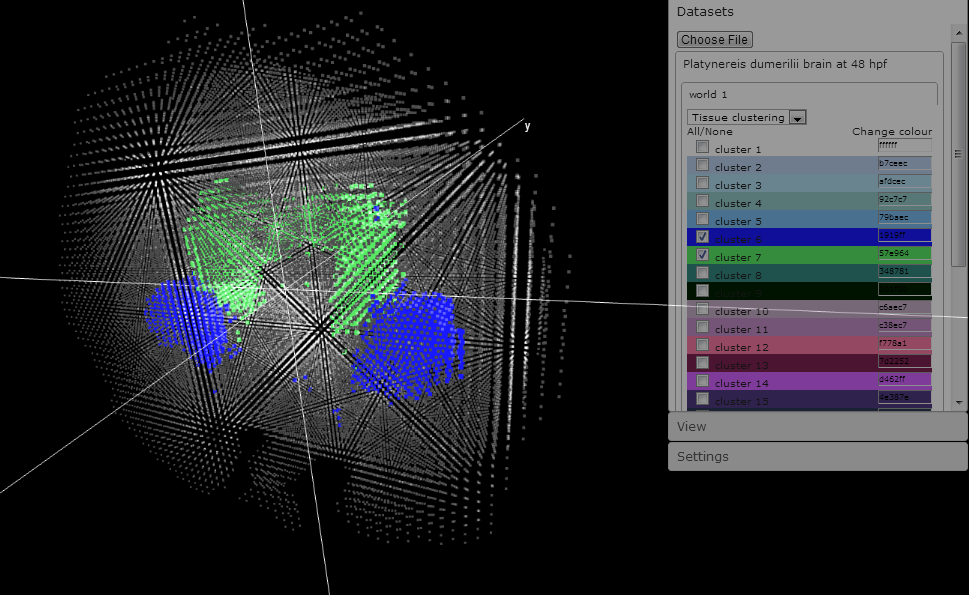
\includegraphics[width=\linewidth]{gfx/chapter3/bioweb3d.png}}
\caption{The 3D location of cells within the brain of the marine annelid \platyfull{} is shown. Two classes are displayed (in green and blue) along with the shadow of the remaining cells. The User interface is visible on the right of the screen and can be hidden. Data for this figure was taken from \cite{Tomer10}, see \ref{ch:background} for a presentation of \platy{} and chapter \ref{ch:singlecell} for detailed presentation the data from \cite{Tomer}.}\label{fig:bioweb3d}
	\end{figure}

	bioWeb3D can be used to visualise datasets derived from a wide variety of biological assays. Examples are shown on the Github wiki \cite{github}, where a 3D representation of a Principal Component Analysis (PCA) carried out with R and the 3D structure of a protein extracted from the PDBe database are displayed.
	
	More generally, the user can interact with the visualisation via an interface on the right of the screen, which contains three panels. In the ``dataset" panel, the user can choose the {\it{datasets}} and {\it{information layer}} files that should be represented in each world. This panel also allows the user to show/hide specific classes of the selected information layers. Each dataset file entered will create a new sub-panel where the user can input {\it{information layer}} files for that world. Selecting an {\it{information layer}} in the drop-down list will display the data in the current world and generate a list of classes that the user can modify regarding their visibility and colour. The ``View" panel enables the user to choose which of the worlds are shown on the screen, ranging from 1 to 4. Finally, the ``Settings" panel provides the user with a number of options that affect all worlds and all datasets, such as modifying the axes scales, modifiying the transparency and size of raw data points and information layer coloured points. The user can also choose to enable centering of the data around 0 or leave the coordinates as inputted.

		\paragraph{bioWeb3D and local software}
Many 3D visualisation software tools, most of which require local installation, exist and provide similar functionalities with standard 3D format input such as Wavefront .OBJ. Some are extremely generic and powerful like Blender or Amira 3D. However, these tools are not typically oriented towards a scientific audience. Moreover, those that are more focused on science are often targeted towards a very specific application, especially in the medical sciences \cite{Wang093D}. In this context, I believe that bioWeb3D can be useful as it is completely generic and browser based. It should also be noted that recent browser improvements regarding GPU acceleration through the WebGL paradigm allow bioWeb3D to visualise several hundred thousand points. Additionally, local software is usually platform specific, which is not the case for browser based applications.

		\paragraph{bioWeb3D and Java Applets}
As mentioned previously, browser based 3D visualisation tools currently exist mainly in the form of Java Applets. This technology has attracted much criticism in 2012 regarding security flaws, leading the ``United States Computer Emergency Readiness Team" to advise that all Java Applets should be disabled due to current and future Java vulnerabilities \cite{security}. The development of WebGL technology is viewed by many as a candidate for replacing Applets. 



		\paragraph{Current limitations}
The main current limitation of a WebGL based application is the machine and browser compatibility. Only computers with fairly recent graphic cards will be able to run a 3D environment. It should also be noted that Microsoft has notified the developer community that Internet Explorer is not scheduled to support WebGL in the near future. However, importantly, Chrome, Firefox, Safari and Opera all now support WebGL applications. Moreover, WebGL is also supported on mobile platforms such as iOS or Android. \cite{caniuse}


		\paragraph{Open source and collaborative development}
As a fully open source software, the source code for bioWeb3D is available on Github \cite{github}, a web platform that allows interested parties to collaborate on the development of the project. In the wiki page ``Contribute to bioWeb3D", directions to alter or add capabilities to bioWeb3D are provided for users who wish to get involved.

	\subsection{Conclusions}
bioWeb3D is designed to be a simple and quick way to view 3D data with a specific focus on biological applications.  Being browser-based, the software can be easily used from any computer without the need to install a piece of software. Importantly, bioWeb3D has been designed to offer a very straightforward and easy-to-use working environment. Despite current limitations in terms of compatibility or rendering performance for large numbers of points, I believe that bioWeb3D will enable non-experts in 3D data representation to quickly visualise their data and the information attached to it in many biological contexts, thus facilitating downstream analyses.

	\subsection{Availability and requirements}
The full source code is available on the Github page of the project \cite{github}. A live version of the software is online \cite{bioWeb3D}. You will require a graphical card and a browser with WebGL capabilities to run bioWeb3D.

\section{Non spatial clustering methods}
	\subsection{Hierarchical clustering}
    - General description of the method
    - Computing distance matrix on binary expression data
    - Hclust method to use (full or partial)
    - Discuss the choosing the K with hClust (dendrogram is not informative)
 
	\subsection{Independent mixture models}
    - General statistical framework
    - Present the model
    - Gene independence hypothesis (this will be discussed further in the next chapter)
    - Likelihood of the model
    - EM algorithm to maximize the parameters (theta)
    - Choosing K with the BIC

\section{Discussion}
	\subsection{Spatial clustering techniques (hierarchical, model based)}
    - Limits of non spatial methods on noisy data (cite the "cell model of chapter 1" paragraph)
    - Not using the spatial data seems silly when we do have it (playing chess blind comparison ?)
    - Some clustering methods are able to take into account the spatial localization of the data points as well as the expression data
    - Quickly present spatial methods (spatial hclust), Mixture with a spatial component

	\subsection{Method chosen}
    - MRF because theta parameters are informative, easy to compute a likelihood and to choose K




%*****************************************
%*****************************************
%*****************************************
%*****************************************
%*****************************************
